\chapter{Opis projektnog zadatka}
		
		\indent Cilj ovog projekta je razviti programsku podršku za stvaranje web aplikacije "Eventko". Ova aplikacija omogućit će korisnicima da kvalitetnije i jednostavnije stvaraju i upisuju se na događaje. Aplikacija će pružati uvid u sve trenutne javne događaje kojima se može pristupiti. Događaji će biti prikazani u obliku kalendara koji je inspiriran izgledom kalendara u aplikaciji Ferko. \\
			
		\indent Prilikom prvog pokretanja aplikacije korisnik se nalazi na stranici za prijavu na kojoj će se prikazati prozorčić s poljima za potrebne podatke:
		
		\begin{packed_item}
			\item polje za unos korisničkog imena profila
			\item polje za unos lozinke korisničkog profila
			\item gumb za prijavu
			\item gumb za izradu novog računa (\textit{sign up})
		\end{packed_item}
		
		\indent Tijekom prvog pokretanja profil još nije napravljen tako da je potrebno stisnuti gumb \textit{Izradi račun} kako bi se napravio novi korisnički profil. Nakon pritiska gumba aplikacija prebacuje korisnika na novu stranicu na kojoj je prikazan prozor s poljima za unos potrebnih podataka za izradu novog profila, kao i gumbi za registraciju ili za povratak na stranicu za prijavu. Za registraciju novog profila potrebni su sljedeći podaci:
		
		\begin{packed_item}
			\item korisničko ime
			\item nadimak (neobavezno)
			\item lozinka
			\item ponovljena lozinka
			\item e-mail adresa
		\end{packed_item}
	
		\indent Nakon što su podaci uspješno uneseni potrebno je stisnuti gumb "Izradi" kako bi se novi korisnički profil generirao. Po uspješnom stvaranju korisnik je prebačen natrag na stranicu za prijavu te se može prijaviti svojim novim korisničkim računom. Nakon uspješne prijave aplikacija vodi korisnika na početnu stranicu.
		\eject
		
		\indent Na početnoj stranici prikazana je alatna traka na kojoj su redom nanizani sljedeći objekti:
		
		\begin{packed_item}
			\item logotip aplikacije Eventko
			\item Obavijesti
			\item Moji prijatelji
			\item Pohađani događaji
			\item Moj profil
			\item Odjava
		\end{packed_item}
	
		\indent Ispod alatne trake prikazan je gumb \textit{Stvori novi događaj} kojim je moguće kreiranje novog javnog ili privatnog događaja te osobne obaveze. Odabir otvara novi prozorčić u koji je potrebno napisati sljedeće podatke:
		
		\begin{packed_item}
			\item Vrsta događaja
			\item Naslov
			\item Lokacija (omogućen prikaz na Google Kartama uz API)
			\item Datum i vrijeme
			\item Oznake događaja (npr. kava, učenje, društvene igre...)
			\item Opis događaja
		\end{packed_item}
	
		\indent Ispod gumba \textit{Stvori novi događaj} nalaze se liste aktivnih korisnika te istaknutih događaja koje uređuju moderatori. Većinu prikaza stranice zauzima središnji kalendar na kojem su vidljive sve korisnikove obaveze te događaji kojima je odabrao prisustvovati ili koje sam organizira. Prikazuje se tekući tjedan, a moguće je listati i one nadolazeće. \\
		
		\indent S desne strane nalazi se sekcija \textit{Javni događaji} s gumbom \textit{Izbornik} koji otvara padajući izbornik s nadolazećim javnim događajima u kojima je moguće sudjelovati. Odabir pojedinog događaja privremeno ga prikazuje u kalendaru te su klikom na njega vidljive osnovne informacije i oznake, kao i opcija prijave čime je dodan u korisnikov kalendar. \\
		
		\indent Odabir kartice \textit{Obavijesti} prikazuje listu obavijesti inicijalno poredanih od najnovijih prema starijim. Korisnik može biti obaviješten da je privremeno ili trajno suspendiran, promaknut u moderatora i slično.
		\eject
		
		\indent Odabir kartice \textit{Moji prijatelji} otvara stranicu koja prikazuje listu trenutnih prijatelja korisnika, a s desne strane nalazi se gumb za pretraživanje korisnika po korisničkom imenu te gumb za dodavanje prijatelja pomoću QR koda. \\
		
		\indent Odabir kartice \textit{Pohađani događaji} prebacuje korisnika na novu stranicu sa svim događajima na kojima je korisnik sudjelovao i bit će mu omogućeno da ih označi sa \textit{Sviđa mi se} ili \textit{Ne sviđa mi se}. \\
		
		\indent Odabir kartice \textit{Moj profil} otvara stranicu koja prikazuje korisnikove podatke:
		
		\begin{packed_item}
			\item nadimak, uz opciju izmjene
			\item korisničko ime
			\item e-mail adresa
			\item jedinstveni korisnički QR kod
			\item ukoliko je riječ o običnom korisniku, opcija pretplate za Premium račun
		\end{packed_item}
		
		\indent Odabir kartice \textit{Odjava} vraća korisnika na stranicu za prijavu. \\
		
		\indent Različite uloge u aplikaciji su sljedeće:
		
		\begin{packed_item}
			\item Običan korisnik
			\item Premium korisnik
			\item Pregledavač
			\item Moderator
			\item Administrator
		\end{packed_item}
	
		\indent Pregledavač je korisnik na uvodnoj stranici za prijavu koji trenutno nije prijavljen. Običnom korisniku dostupne su sve funkcionalnosti prethodno opisane. \\
		
		\indent Premium korisnik ima sve mogućnosti običnoga uz dodatnu opciju promoviranja određenog broja događaja koje organizira, čime se oni prikazuju na listi istaknutih događaja na lijevoj strani stranice. \\
		
		\indent Moderator ima sve mogućnosti premium korisnika, uz to što ima dodatnu karticu na alatnoj traci imena \textit{Upravljanje korisnicima}, koja ga prebacuje na novu stranicu na kojoj može suspendirati korisnike koji se ne ponašaju u skladu s bontonom aplikacije. Također ima opciju \textit{Izmjeni oznake} na događajima kako bi mogao dodati ili ukloniti oznake po potrebi. Konačno, ima opciju \textit{Izbriši event} ako je neki javni događaj neprimjeren. \\
		
		\indent Administrator ima sve mogućnosti moderatora uz to što može na stranici za upravljanje korisnicima ili promovirati posebno vrijedne članove zajednice u moderatore, ili obrisati račune korisnika koji uporno krše pravila i nakon privremene suspenzije.
		
		\section{Primjeri u \LaTeX u}
		
		\textit{Ovo potpoglavlje izbrisati.}\\

		U nastavku se nalaze različiti primjeri kako koristiti osnovne funkcionalnosti \LaTeX a koje su potrebne za izradu dokumentacije. Za dodatnu pomoć obratiti se asistentu na projektu ili potražiti upute na sljedećim web sjedištima:
		\begin{itemize}
			\item Upute za izradu diplomskog rada u \LaTeX u - \url{https://www.fer.unizg.hr/_download/repository/LaTeX-upute.pdf}
			\item \LaTeX\ projekt - \url{https://www.latex-project.org/help/}
			\item StackExchange za Tex - \url{https://tex.stackexchange.com/}\\
		
		\end{itemize} 	


		
		\noindent \underbar{podcrtani tekst}, \textbf{podebljani tekst}, 	\textit{nagnuti tekst}\\
		\noindent \normalsize primjer \large primjer \Large primjer \LARGE {primjer} \huge {primjer} \Huge primjer \normalsize
				
		\begin{packed_item}
			
			\item  primjer
			\item  primjer
			\item  primjer
			\item[] \begin{packed_enum}
				\item primjer
				\item[] \begin{packed_enum}
					\item[] primjer
					\item[b] primjer
				\end{packed_enum}
				\item primjer
			\end{packed_enum}
			
		\end{packed_item}
		
		\indent primjer url-a: \url{https://www.fer.unizg.hr/predmet/proinz/projekt}
		
		\noindent posebni znakovi: \# \$ \% \& \{ \} \_ 
		$|$ $<$ $>$ 
		\^{} 
		\~{} 
		$\backslash$ 
		
		
		\begin{longtblr}[
			label=none,
			entry=none
			]{
				width = \textwidth,
				colspec={|X[8,l]|X[8, l]|X[16, l]|}, 
				rowhead = 1,
			} %definicija širine tablice, širine stupaca, poravnanje i broja redaka naslova tablice
			\hline \multicolumn{3}{|c|}{\textbf{naslov unutar tablice}}	 \\ \hline[3pt]
			\SetCell{LightGreen}IDKorisnik & INT	&  	Lorem ipsum dolor sit amet, consectetur adipiscing elit, sed do eiusmod  	\\ \hline
			korisnickoIme	& VARCHAR &   	\\ \hline 
			email & VARCHAR &   \\ \hline 
			ime & VARCHAR	&  		\\ \hline 
			\SetCell{LightBlue} primjer	& VARCHAR &   	\\ \hline 
		\end{longtblr}
		

		\begin{longtblr}[
				caption = {Naslov s referencom izvan tablice},
				entry = {Short Caption},
			]{
				width = \textwidth, 
				colspec = {|X[8,l]|X[8,l]|X[16,l]|}, 
				rowhead = 1,
			}
			\hline
			\SetCell{LightGreen}IDKorisnik & INT	&  	Lorem ipsum dolor sit amet, consectetur adipiscing elit, sed do eiusmod  	\\ \hline
			korisnickoIme	& VARCHAR &   	\\ \hline 
			email & VARCHAR &   \\ \hline 
			ime & VARCHAR	&  		\\ \hline 
			\SetCell{LightBlue} primjer	& VARCHAR &   	\\ \hline 
		\end{longtblr}
	


		
		
		%unos slike
		\begin{figure}[H]
			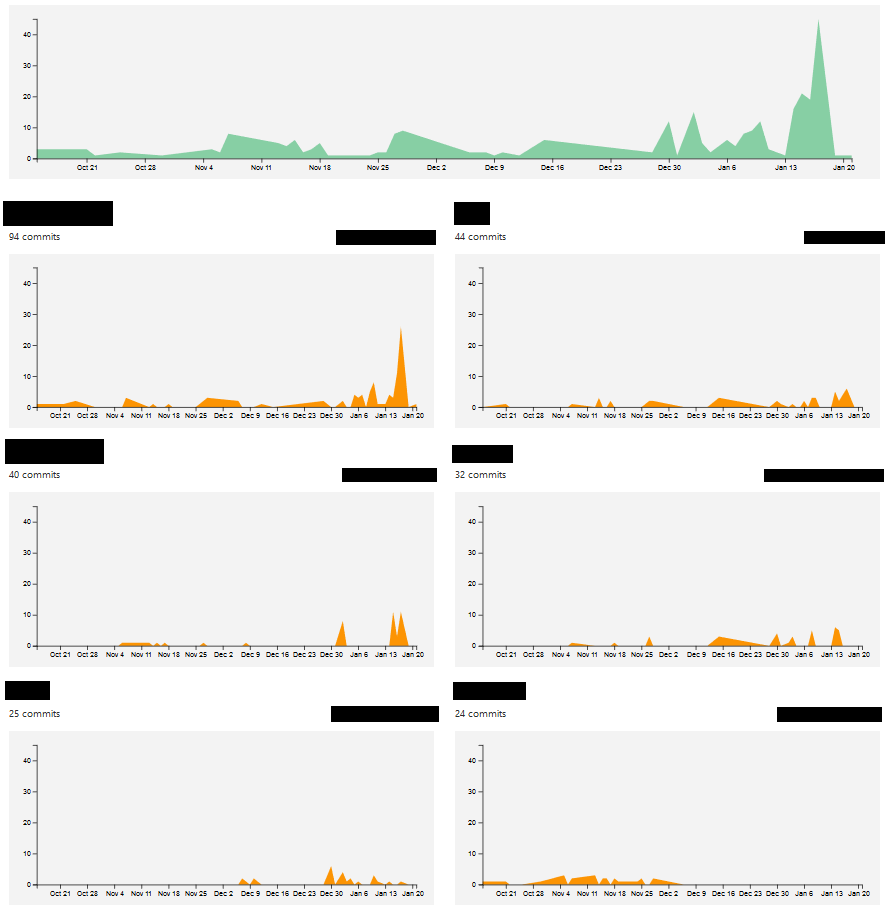
\includegraphics[scale=0.4]{slike/aktivnost.PNG} %veličina slike u odnosu na originalnu datoteku i pozicija slike
			\centering
			\caption{Primjer slike s potpisom}
			\label{fig:promjene}
		\end{figure}
		
		\begin{figure}[H]
			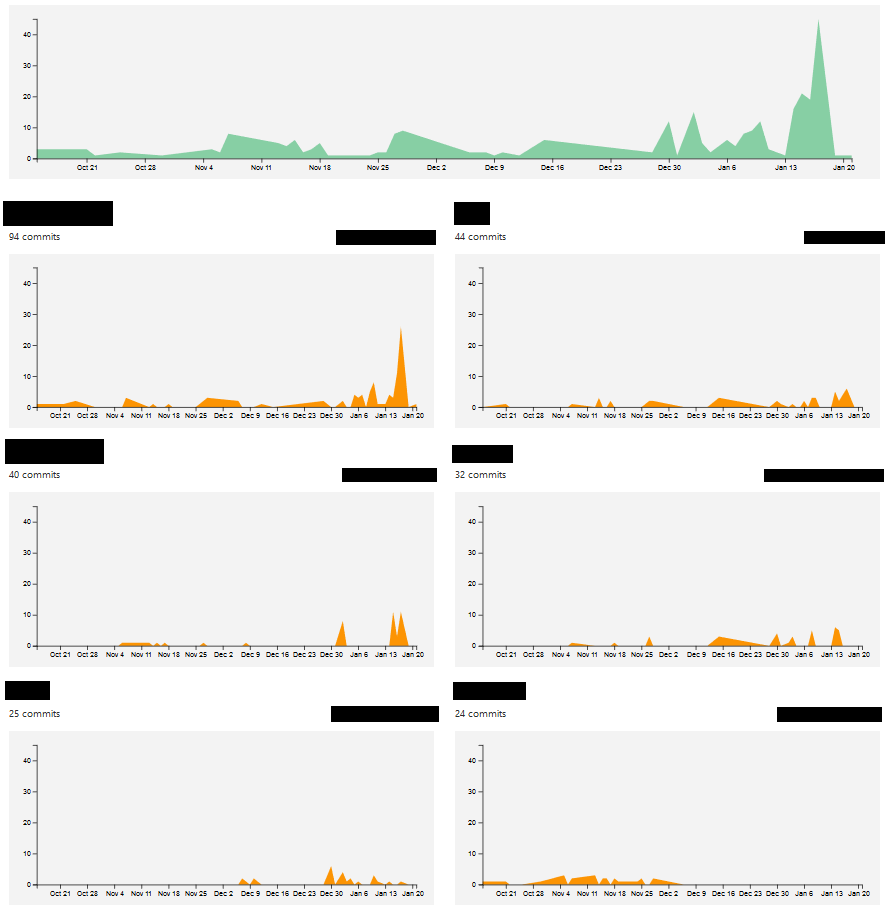
\includegraphics[width=\textwidth]{slike/aktivnost.PNG} %veličina u odnosu na širinu linije
			\caption{Primjer slike s potpisom 2}
			\label{fig:promjene2} %label mora biti drugaciji za svaku sliku
		\end{figure}
		
		Referenciranje slike \ref{fig:promjene2} u tekstu.
		
		\eject
		
	